%===============================================================================
\chapter{Heat transfer}\label{ch02}
%===============================================================================
%
\begin{quote}
\textit{... there is an absolute waste of mechanical energy available to man, when heat is allowed to pass from one body to another at a lower temperature, by any means not fulfilling his} (Carnot's) \textit{criterion of a ``perfect thermo dynamic engine''. As it is most certain that Creative Power alone can either call into existence or annihilate mechanical energy, the "waste" referred to cannot be annihilation, but must be some transformation of energy. ...}

\begin{flushright}
William \citet{Thomson1852energy}, Lord Kelvin (1824–1907) \\
\end{flushright}

\end{quote}
\vspace{1cm}

In this chapter, a brief overview of heat transfer discipline and methods is provided, followed by a review of the most spread strategies for heat transfer control. The focus lies on the control strategies used in this thesis: plasma actuators and jets in crossflow.

\section{Overview of heat transfer processes}
% Definition
The first law of thermodynamics states that energy transport occurs by two basic mechanisms: heat and work transfer. There is no classical definition of heat transfer as a physical phenomenon since this term is commonly used to denote the discipline that studies the exchange of thermal energy through and by matter. A simplified interpretation of heat transfer is given by \citet{bergman2011fundamentals} and reads ``Heat transfer (or heat) is thermal energy in transit due to a spatial temperature difference''. In other words, heat transfer is the thermal energy transport consequence of a temperature difference or gradient.

% Methods
Thermodynamics literature agrees that there are three fundamental heat transfer mechanisms, namely conduction, convection and radiation \citep{bejan1948HT,eckert1959HMT,bergman2011fundamentals,Lienhard2020HT}. If a temperature difference develops on a stationary medium, either a solid or a quiescent fluid, heat transfer occurs via \textit{conduction} across the medium. \textit{Convection}, on the contrary, is the mechanism of thermal energy exchange between the surface of a solid and a moving fluid, or even among the fluid itself when it is moving. Ultimately, \textit{radiation} is the mechanism whereby solid and fluid substances radiate thermal energy to the surrounding space (or other media) in the form of electromagnetic waves. A schematic representation of these mechanisms is provided in figure~\ref{fig:HTmethods} where $q''$ is the heat flux, $T$ is the temperature, $U$ is velocity, and subscripts $\infty$ and $\mathrm{w}$ refer to the free stream and the wall surface, respectively.

\begin{figure}
    \centering
    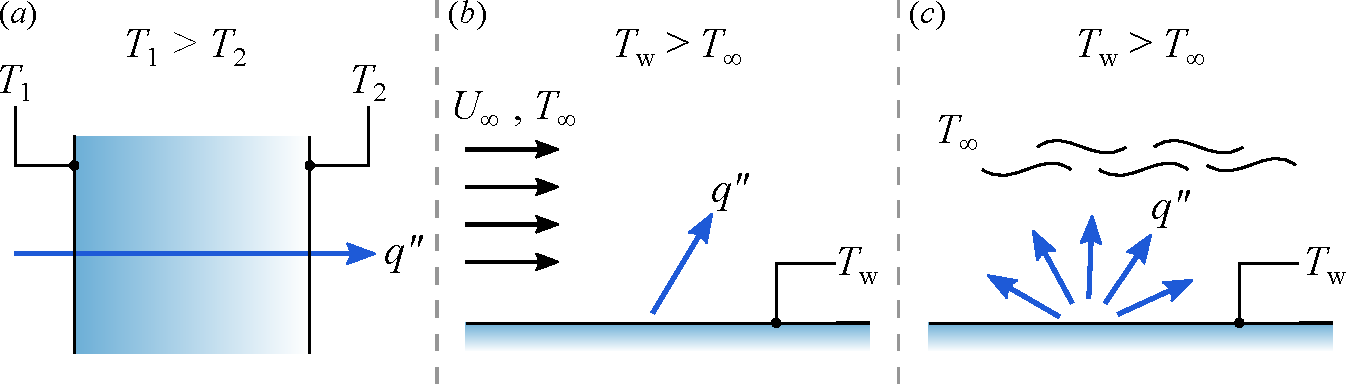
\includegraphics[width = 0.8\linewidth]{figures/dibujo_heat.pdf}
    \caption{Heat transfer mechanisms. (a) Conduction through a solid or a stationary fluid, (b) Convection from a wall to a moving fluid, (c) Radiation from a wall to the surrounding space. Figure adapted from \citet{bergman2011fundamentals}.}
    \label{fig:HTmethods}
\end{figure}

% Convection: the most complex
\citet{Gebhart1971HT} explains that the only physical mechanisms by which heat is transferred through and by the matter are conduction and radiation. However, if conditions occur in a moving medium, as is the case of fluids, the diffusion of thermal energy does not only happen at a microscopic level by the exchange of internal energy among molecules but also by the macroscopic motion of the moving medium. Eventually, this complex process is referred to as convection. Necessarily, convection becomes an additional heat transfer process to explain thermal energy transport in fluid flows. The study of convection includes all the mechanisms of conduction and radiation as well as those of the motion of fluids. Consequently, convection becomes the most challenging of the modes of transport within the field of heat transfer.

% Importance of heat transfer
Heat transfer gathers principles from thermal diffusion, electromagnetic radiation and fluid motion, including theories and knowledge from other branches of science. The study of heat transfer requires the mastery of many concepts and methods of analysis in several disciplines, with a crucial role in countless natural and industrial processes. The impact of thermal energy management on the current socio-economic environment is already discussed in Chapter~\ref{ch01}. Nonetheless, this is not a recent concern of modern science and engineering. In his communication to the Royal Society in 1852 (header of this chapter), Lord Kelvin concludes that there is a universal tendency in nature to the dissipation of mechanical energy, heat transfer being the mechanism driving this process. However, Lord Kelvin did not yet consider the dissipation of energy by convective heat transfer. 

%--------------------------------------------------------------------------------------------------
\subsubsection*{Heat transfer in fluid flows: Convection}

Convection is the heat transfer method of fluids par excellence. Depending on the nature of the fluid motion, convection may be classified into two different types. On the one hand, \textit{forced convection} occurs when the fluid motion is induced by external sources, such as a pump, a blower or the atmospheric wind. Forced convection is the predominant kind in both natural and industrial processes, as is the case of wall-bounded flows, jet shear layers or atmospheric flows. On the other hand, \textit{natural convection} happens when the motion is a direct consequence of buoyancy effects due to the temperature-induced density change within the fluid. A classic example of natural convection is the so-called Rayleigh–Bénard convection \citep{Bodenschatz2000RBC}.
%As an example, \citet{sanmiguelvila2016hconv} studied the onset of horizontal convection experimentally by differential heating on the bottom wall of an encapsulated fluid, and \citet{Shishkina2011Rayleight} applied model-free control strategies to control RBC in a two-dimensional domain. 
% From a flow-control standpoint,

This work focuses on the forced convection in wall-bounded flows, in which the mainstream exchanges energy with the wall surface, as depicted in figure~\ref{fig:dibujo_ThBL}. Two essential concepts are to be introduced, namely the boundary layer and turbulence. As defined in Chapter~\ref{ch01} and expanded in Chapter~\ref{ch04}, turbulence is a flow regime characterised by its nonlinear, chaotic and high-dimensional nature. Additionally, the \textit{boundary-layer} (BL) concept is the baseline of modern fluid mechanics, developed by Ludwig Prandtl in 1904 \citep{prandtl1904BL}. Upon the motion of fluid over a solid surface, a thin layer of air develops at the interface in which the fluid adjusts its velocity from that of the free stream to that of the solid. This region is characterised by strong velocity gradients along the wall-normal direction; hence, viscous effects dominate the flow. This region is commonly known as hydrodynamic, or velocity, boundary layer, and its thickness is denoted by $\delta$. 
Similarly, for incompressible flows, the thermal BL develops when the wall temperature $T_\mathrm{w}$ differs from that of the free stream $T_\infty$, inducing a temperature gradient normal to the wall. The development of velocity and thermal boundary layers is driven by momentum and thermal diffusivity, which are related by a dimensionless group named the Prandtl number ($\nPr$), which relates the kinematic viscosity $\nu$ and the thermal diffusivity $\alpha$ as
\begin{equation}
    Pr = \frac{\text{Momentum diffusivity}}{\text{Thermal diffusivity}} = \frac{\nu}{\alpha}
\end{equation}

The Prandtl number can be used to determine the relation between velocity and thermal BL thicknesses ($\delta$ and $\delta_t$, respectively). As illustrated in figure~\ref{fig:dibujo_ThBL}, for $\nPr >1$, $\delta > \delta_t$, meaning that the flow is dominated by the diffusion of momentum whereas for $\nPr < 1$, the flow is dominated by thermal diffusion so that $\delta < \delta_t$.

\begin{figure}
    \centering
    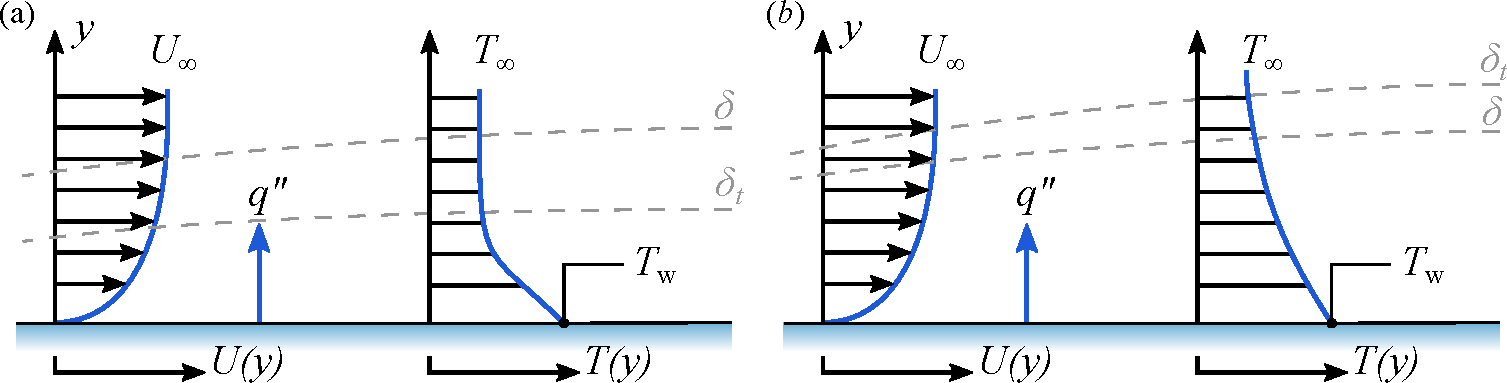
\includegraphics[width = 0.8\linewidth]{figures/dibujo_ThBL.pdf}
    \caption{Boundary layer development on a flat plate with convective heat transfer. (a) Thermal boundary layer thinner than the velocity boundary layer ($Pr > 1$); (b) Thermal boundary layer thicker than the velocity boundary layer ($Pr < 1$). The symbols correspond to wall-normal coordinate $y$, wall temperature $T_\mathrm{w}$, heat flux from the wall $q''$, and freestream velocity and temperature $U_\infty$,$T_\infty$, respectively.}
    \label{fig:dibujo_ThBL}
\end{figure}

Recalling the definition by \citet{Gebhart1971HT}, discussed above, convection is comprised of the energy dissipation due to random molecular motion and the bulk energy transfer due to the motion of the fluid at a macroscopic scale. These mechanisms are referred to as \textit{diffusion} and \textit{advection}, respectively. In turbulent boundary layers (TBLs), advection is dominated by the motion of coherent structures. From a thermodynamical perspective, coherent structures can be defined as fluid volumes moving collectively and with similar thermodynamic properties. The molecules composing the coherent structures retain their random motion through which diffusion is accomplished; hence the total thermal energy transport results from the superposition of random molecular motion on the microscopic scale and bulk fluid motion on the macroscopic scale. In other words, convective heat transfer is the cumulative effect of diffusion and advection. Diffusion is predominant in the near-wall region, where large eddies vanish into smaller scales dissipating energy. At the surface boundary, where the flow velocity adjusts to that of the wall, heat is transferred by diffusion only. The bulk energy transport is carried out by large structures within the boundary layer, exchanging heat with the free stream as well.

Regardless of the nature of the convection heat transfer process, the convective heat flux $q''~(\mathrm{W/m}^2)$ between the fluid and the boundary surface is determined from Newton's law of cooling, namely
\begin{equation}\label{eq:Newton_cooling}
    q'' = h(T_\mathrm{w} - T_{\mathrm{aw}})
\end{equation}
where the parameter $h~(\mathrm{W/m}^2\cdot\mathrm{K})$ is referred to as the convection heat transfer coefficient, and $T_{\mathrm{aw}}$ is the adiabatic wall temperature. The adiabatic wall temperature is a reference temperature of the fluid at which the heat transfer between the fluid and the wall is null. Its value depends on the flow conditions. For incompressible flows, as considered throughout this dissertation, the adiabatic wall temperature practically coincides with that of the undisturbed stream, i.e. $T_{\mathrm{aw}} \approx T_\infty$. Instead, for compressible flows, the reader is referred to \citet{Germain1955taw}, in which an extensive analysis and formulation are available.

Equating the heat conducted from the wall by the fluid by Fourier's law of thermal conductivity to the same heat transfer expressed in terms of a convection mechanism by Newton's law of cooling, the following relation is achieved:
\begin{equation}\label{eq:cond_conv}
    -k \left. \frac{\partial T}{\partial y} \right|_{y = 0} \equiv h(T_\mathrm{w}-T_\infty)
\end{equation}
where $k$ is the thermal conductivity of the fluid. The left-hand side in Eq.~\eqref{eq:cond_conv} represents the heat removed from the wall since no fluid flows through the wall. This relation can be expressed in dimensionless form as
\begin{equation}\label{eq:Nu}
    \left. \frac{\partial \left( \frac{T_\mathrm{w}-T}{T_\mathrm{w}-T_\infty}\right)}{\partial (y/\ell)} \right|_{y/\ell = 0} = \frac{h\ell}{k} \equiv \nNu_\ell.
\end{equation}
being $\ell$ a characteristic length of the flow under consideration, and $\nNu_\ell$ the Nusselt number based on $\ell$. The Nusselt number, as defined in Eq.~\eqref{eq:Nu}, may be interpreted as the ratio of heat transfer rate by convection to that of pure conduction through the medium. This dimensionless group is a classical form to refer to the convective heat transfer; however, it must not be mistaken with the Biot number ($\nBi = h\ell/k_\mathrm{w}$, being $k_\mathrm{w}$ the thermal conductivity of the solid wall), which is the ratio of the internal conductive resistance of a solid to the boundary layer convective resistance.

The study of convective heat transfer in fluid flows reduces to the determination of $h$. For experimental investigations, measuring heat fluxes at the wall requires both heat-flux sensors and temperature transducers. Papers 2, 3 and 5 in Part II of this manuscript, rely on the same methodology consisting of a heated-thin-foil sensor together with infrared thermography to acquire temperature. The heated-thin-foil is thermally thin \citep{astarita2012infrared}, i.e. it can be considered isothermal across its thickness since the Biot number is small for all the proposed problems ($\nBi < 0.1$). This non-intrusive measurement technique captures the distribution of convective heat flux on a surface. The interested reader is referred to the methodology section of Papers 2, 3 and 5 in Part II. 
%the Fourier number ($\nFo = \alpha_{s}/fs_{s}^2$, where $\alpha_{s}$ is the thermal diffusivity of the sensor, $s_{s}$ is the sensor thickness and $f$ is the IR camera sampling frequency, much larger than the inverse of the time scale of the phenomenon) is larger than unity; consequently, according to [20] the temperature distribution along the thickness of the printed circuit board is linear.
%-----------------------------------------------------------------------------------------
\subsubsection*{Analogy between Momentum and Heat Transfer}

The transport of momentum and energy in turbulent flows is based on similar mechanisms. The transport equations of these two quantities resemble each other. In their dimensionless form, the equations are analogous, depending on a few parameters, namely the Reynolds number \nRe, the Prandtl number \nPr, and the Nusselt number \nNu~(or the Stanton number \nSt, later introduced). There exist several versions of the momentum and heat transfer analogy. The most relevant are briefly described below, avoiding the mathematical process to obtain them for brevity. The interested reader is referred to the wide variety of textbooks on heat and mass transfer that cope with this topic \citep[\eg][]{bergman2011fundamentals,Lienhard2020}.

The first attempt to formulate this similarity was the famous Reynolds analogy. \citet{reynolds1874analogy} suggested that the concentration, velocity and temperature distributions should have a similar form, proposing a simplified mathematical rule that relates momentum and heat transfer processes.
\begin{equation}\label{eq:Re_analogy_aux}
    \frac{h}{\rho U_\infty c_p} = \frac{1}{2}\frac{\tau_w}{1/2\rho U_\infty^2}
\end{equation}

The right-hand side in Eq.\eqref{eq:Re_analogy_aux} represents the dimensionless representation of the wall shear stress $\tau_w$ (the Fanning friction factor $f = 2\tau_w / \rho U_\infty^2$), whereas the left-hand side of Eq.\eqref{eq:Re_analogy_aux} is a dimensionless group referred to as the Stanton number (\nSt) that measures the ratio of heat transferred to the fluid ($h$) to the fluid thermal capacity ($\rho U_\infty c_p$ being $\rho$ the fluid density, $U_\infty$ its velocity, and $c_p$ its isobaric specific heat). In other words, \nSt~describes the relationship between the heat transfer and the shear force at the wall, which translates into a geometric similarity between the velocity boundary layer and the thermal boundary layer. Hence, the Stanton number directly refers to $\nNu$, $\nPr$ and $\nRe$, relating momentum and thermal processes. The definition and physical interpretation of the Stanton number reads
\begin{equation} \label{eq:Stanton}
    \nSt = \frac{\text{Actual heat flux to the fluid}}{\text{Maximum possible enthalpy change}} = \frac{h\cancel{\Delta T}}{\rho U_\infty c_p\cancel{\Delta T}} = \frac{\nNu}{\nPr\nRe}
\end{equation}

Developing Eq.\eqref{eq:Re_analogy_aux}, Reynolds' analogy in its classical form reads as
\begin{equation}\label{eq:Re_analogy}
    \nSt = \frac{f}{2} \qquad \text{Reynolds analogy \citep{reynolds1874analogy}}
\end{equation}

Similarly, \citet{prandtl1910beziehung}, unaware of the pioneering work by \citet{reynolds1874analogy}, pointed out that the velocity and temperature differential equations are identical when the thermal and momentum diffusivities are equal. Both Reynolds' and Prandtl's analogies are valid for the simplified case of a boundary layer that develops on a flat plate under zero-pressure-gradient (ZPG) conditions and in the limit of $\nPr = 1$. Soon an unsuccessful attempt by \citet{taylor1916conditions} tried to formulate a generalized analogy for cases with $\nPr \neq 1$. \citet{colburn1933analogy} explored the relevance of the Prandtl number on the turbulent transport similarity. By combining energy and momentum transport equations within a turbulent boundary layer on a flat plate, the group $\nSt\nPr^{2/3}$ arises, which is defined as the $j$-factor. This analogy is an extension of classical Reynold's analogy, which is commonly known as the $j$-factor or Chilton-Colburn analogy \citep{Chilton1934Jfactor},
\begin{equation}\label{q:jfacto_analogy}
    \frac{f}{2} = j = \nSt\nPr^{2/3} = \frac{\nNu}{\nRe\nPr^{1/3}}
\end{equation}

The validity of these analogies is nonetheless restricted only to the boundary layer flow on a flat plate under ZPG conditions. Several authors aimed at developing more general models to relate heat and momentum transport; however, most of them rely on empirical coefficients or are case-dependent. For the reader's interest, an extensive review of heat-momentum analogies is presented by \citet{churchill1997critique}. %The above discussion is intended to present to the reader the concept of the heat and momentum transfer analogy, the principle of similarity between these two mechanisms and the definition of the Stanton number. Understanding these concepts enables exploring solutions for heat transfer control in other fields such as skin-fiction reduction, mixing enhancement or wake suppression. Furthermore, Paper 1 in Part II of this thesis leverages the Reynolds analogy to investigate an approach to reducing heat transfer in turbulent boundary layers.

%================================================================================================
%- Heat transfer control:
%================================================================================================
\section{Strategies for heat transfer control}

Heat transfer control is the discipline that explores thermal management strategies with the target of altering the mechanisms behind thermal energy transport. This discipline is commonly known as \textit{heat transfer enhancement} since most efforts are aimed at increasing the heat transfer capabilities of the system. Heat transfer enhancement is present in many industrial and research areas, such as space satellites' thermal management by radiation, conduction mechanisms in solar panels or convective heat fluxes in heat exchangers of engines. In this section, the focus lies on convective heat transfer control, performance quantification criteria, and the strategies to achieve enhancement. 

For an enhanced surface in single-phase flows, the ``basic performance characteristic'' is the $j-$factor from the Chilton-Colburn analogy, together with the friction factor, $f$, as a function of the Reynold number, $\nRe$. A straightforward possibility to quantify the performance enhancement is to calculate the ratios $j/j_0$ and $f/f_0$, where the subscript $0$ is for the reference condition. Although it depends on the enhancement strategy in use, commonly $f > f_0$ under the same $\nRe$. Thus, this approach does not accurately quantify the actual performance improvement, subject to specific operating constraints. Considering $j/j_0$ may yield unfair comparisons since the enhanced flow condition is allowed to operate at a higher pressure drop than the reference. In other words, the reference flow condition could achieve higher $h$ if operated at higher $\nRe$ to balance the pressure drop to that of the enhanced case. Therefore, the additional energy required to promote the enhanced heat transfer condition must be quantified to determine the performance fairly.

In the literature, there exist several measures of \textit{performance} for heat transfer enhancement strategies. It is worth noting that heat transfer enhancement is a discipline strongly related to the design, study and optimisation of heat exchangers. Based on the discussion by \citet{manglik2003heat}, the performance evaluation criteria (PEC) for single-phase flows strongly depend on the objective of the enhancement. A general formulation is proposed by both \citet{manglik2003heat} and \citet{webb2005enhanced} that relates the change in heat transfer coefficient $h$ for a heat transfer surface $A$ with the required pumping power $P$. This classical interpretation for heat transfer enhancement reads,
\begin{equation}\label{eq:PEC}
    \frac{hA/h_{0} A_{0}}{(P/P_{0})^{1/3}(A/A_{0})^{2/3}} = \frac{j/j_{0}}{(f/f_{0})^{1/3}},
\end{equation}
The general PEC is driven by the three variables on the left-hand side, namely ($hA/h_0A_0$), ($P/P_0$), and ($A/A_0$). By setting one of the variables as the objective, the remaining two are considered operating constraints, fixing their values to 1.0. In this work, the PEC in Eq.~\eqref{eq:PEC} is adjusted to the case of a turbulent boundary layer flow in which the thermal energy transfer process is mainly driven by a change in temperature between the mainstream and the wall. Consequently, the heating/cooling area and the Reynolds number are unaltered when applying the heat transfer enhancement technique, $A/A_0 = 1$. Therefore, the main objective of the herein considered problems is to control the value of $h$, while the power requirement is envisioned as a penalty term in the objective function. A deeper discussion on the formulation of the optimisation problem is provided in Chapter~\ref{ch03}.

The heat transfer control problem is then classified into different categories, depending on whether the objective is to enhance or reduce heat transfer and on the type of control strategy in use. For the latter, literature differentiates between \textit{passive} and \textit{active} techniques \citep[\eg][]{webb2005enhanced}. Passive flow control techniques are those that perform the actuation regardless of an external power supply. This is commonly achieved by geometry alteration of the surface such as roughness elements \citep{Hwang1995roughness,Hechuan2018ratchet}, obstacles \citep{mallor2018cubes}, riblets \citep{Mallor2019ribPOD}, or vortex generators \citep{Awais2018review,Ke2019VG}. Despite the undoubted effectiveness of passive elements, these devices are constantly present in the flow field, inducing a continuous pressure drop that translates into an undesired skin-friction augmentation. The inability to trigger the control action when desired or to adjust the control authority also deteriorates the performance of passive elements. Active control techniques cope with all the enumerated weaknesses at the cost of an external power supply to perform the actuation on the flow. There are countless active flow control devices such as continuous \citep{puzu2019jet} or synthetic \citep{Giachetti2018synjet} jets in crossflow, plasma actuators \citep{roy2008plasma}, electromagnetic forcing \citep{Kenjere2008EMheat} or moving walls by electroactive materials \citep{Leal2013rev_electroactive}, to name a few. Active control has gained interest in the flow control and heat transfer communities during the last decades due to its outstanding versatility in the control design, from the actuator to its control logic. Furthermore, the incursion of sophisticated algorithms into flow control triggers the possibility of exploring unconventional flow control strategies, adjusting their authority upon the requirements of the flow according to a pre-stated objective.

In this work, the focus lies on a specific mechanism through which heat transfer enhancement is achieved in turbulent flows, which consists of inducing streamwise vortices embedded in the boundary layer \citep{jacobi1995}. The resulting near-wall coherent structures prevail over a significant downstream distance, promoting cross-stream momentum transfer within the boundary layer. This actuation facilitates the transport of high-momentum fluid from the outer region towards the wall, exacerbating heat transfer and turbulent mixing. Classical, passive heat transfer enhancement methods exploiting this principle are wall-mounted obstacles and vortex generators. 
%For the latter, there are three basic recommendations to design the VG: longitudinal vortices are more effective than transversal vortices; (2) delta winglets outperform rectangular winglets; and (3) optimum angles of attack lies in the range $[30^\circ,45^\circ]$.
Vortex generators (VG) are widely used in the aeronautical industry as a passive element to promote turbulence transition on adverse-pressure gradient flows \citep{Lin2002reviewVG} and in heat transfer enhancement applications such as heat exchangers \citep{Awais2018review}.  Regarding wall-mounted obstacles, the work by \citet{Chyu1996obstacles} investigates the flow topology and heat transfer distribution around several obstacle shapes. A horseshoe vortex develops upstream with the corresponding streamwise counter-rotating vortex pair extending downstream at both sides. At the downstream side of the obstacle, the flow separates and recirculates, yielding a reduction of convective heat transfer at the wall. The flow re-attaches further downstream with an impinging flow known as the arch-shaped vortex. According to \citet{Chyu1996obstacles}, the cubes are the best shape for heat transfer enhancement purposes upstream of the obstacle. However, they present a strong recirculation area as demonstrated by \citet{nakamura2001cube}. \citet{mallor2018cubes} aimed to solve this issue by perforating the wall-mounted cubes similar to the perforated fins in channel flow used by \citet{Hwang1995roughness}. Perforated cubes not only reduce the recirculation region but also increase the maximum Nusselt number at the wall due to the impingement of the flow coming through the perforation. It is worth noting that the flow around an obstacle resembles that induced by other active elements as the jets in cross flow \citep{fric_roshko_1994}. A detailed description of jets in cross flow reads in section~\ref{ss:JICF}.

On the contrary, few contributions exist regarding heat transfer reduction in turbulent boundary layers. The early and extensive study by \citet{Moffat1984review} investigates a TBL when submitted to different perturbations such as acceleration, deceleration, roughness and surface curvature, among others. Although this study may seem obsolete, it pointed out several basic flow mechanisms to modify the Stanton number that have been later better explained and exploited for flow control, such as the opposition control \citep{Choi1994}. In that respect, the contributions in skin-friction drag reduction are counted by hundreds, which could be extrapolated to convective heat transfer reduction by invoking the analogy between momentum and heat transfer described above. Most effective flow control techniques to reduce momentum flux must interrupt the bursting cycle's self-sustaining regenerative process \citep{hamilton1995,Jimenez1999,schoppa2002}. Typically, the cycle envisions the generation of low-speed streaks by the lift-up effect of fast-advecting streamwise vortices \citep{Butler1993streak} within the boundary layer. Then, the transient growth of the streaks collapses in the regeneration of streamwise vortices \citep{hamilton1995,schoppa2002}. The so-called opposition control \citep[\eg][]{Choi1994,Stroh2015,Fukagata2003oppcontrol} is the most classical approach used to reduce skin-friction drag, which aims at damping coherent structures in the near-wall region. Another classical approach is the generation of embedded streamwise vortices within the turbulent boundary layer, as proposed by \citet{Schoppa1998}. A 20\% drag reduction in a turbulent channel upon generating large-scale counter-rotating streamwise vortices by wall jets. In contradiction to the above discussion for heat transfer enhancement, the large-scale swirl motion merges streaks into a larger streak envelope with reduced strength, thus cancelling the generation of streamwise vortices in the last part of the bursting cycle and reducing drag \citep{schoppa2002}. The heat transfer footprint of streamwise vortices embedded in a TBL is investigated by \citet{Zhang1993heatJICF}, concluding that those vortices that are deeply embedded with a reduced size and strength are the ones that could be used to reduce heat transfer and skin friction. Similar experimental investigations use jets vortex generators \citep{iuso2002} or body forces by plasma actuators \citep{cheng_wong_hussain_schroder_zhou_2021} to induce large-scale vortical motion that effectively reduces skin-friction drag.\\

The following sections provide a detailed description of the active flow control techniques used in this thesis. Plasma actuators are employed in Paper 2 to reduce heat transfer whereas jets in cross flow are tuned in Papers 3 and 5 to maximise the convective heat transfer.

%------------------------------------------------------------------------------------------
\subsection{Plasma actuators}\label{ss:PA}

The term \textit{Plasma} was first coined by \citet{Langmuir1928plasma} to denote an electrically-neutral ionised gas. Since then, the term plasma has been used in physics to define when substances feature charge equilibrium, generally known as the \textit{fourth state of matter}. Hence, plasma is a gaseous system of free-floating charged species that mutually interact, providing outstanding electromagnetic response of the plasma cloud and good electrical conductivity. The study of plasma and its applications have received overwhelming attention in the past, especially in flow control, space propulsion, material science and medicine, among others. The interested reader is referred to the extensive work by \citet{fridman2008plasma} to delve into plasma physics.

The production and preservation of a plasma discharge come hand in hand with several technological challenges due to the considerable energy requirement for promoting gas ionisation and the degradation of materials nearby the plasma cloud. The ionisation of a given volume of gas is usually achieved by applying an electric field, which is generated by either direct current (DC) or alternating current (AC) voltage. There is a minimum required voltage to sustain electron-ion pairs in the gas, the \textit{breakdown voltage} $E_b$, which depends on several factors like the driving frequency, the temperature and pressure of the gas, or the chemical composition of the gas \citep{Kunhardt1980breakdown,kunhardt1983electrical}. For the particular case at standard atmospheric conditions using air as a gas, the produced plasma is characterised by incomplete ionisation and no thermal equilibrium. Hence, the energy provided by the electric field is mainly stored in the free electrons, which translates into a relatively low temperature, given the name of \textit{cold plasma} \citep{Yamamoto2007plasma}. This kind of plasma is typically used in flow control applications as later proposed in this thesis.

The plasma actuators are devices that generate plasma to induce body forces in a specific manner. According to the extensive review by \citet{Kotsonis2015review}, plasma actuators are the modern technological implementation of Aristotle's concept of the \textit{unmoved mover}. The plasma actuator is a static device that can induce motion in the surrounding fluid without moving parts or the injection of a secondary stream. There are several alternatives for plasma actuators such as alternating current dielectric barrier discharge (AC-DBD) \citep{Roth1998dbd}, direct current corona (DC-corona) \citep{Leger2001corona}, nanosecond pulsed dielectric barrier discharge (ns-DBD) \citep{Roupassov2009nsplasma}, and arc filament actuators \citep{Samimy2004arcfilament}. In the following, only AC-DBD plasma actuators are considered, which is the kind used in this thesis.

\begin{figure}
    \centering
    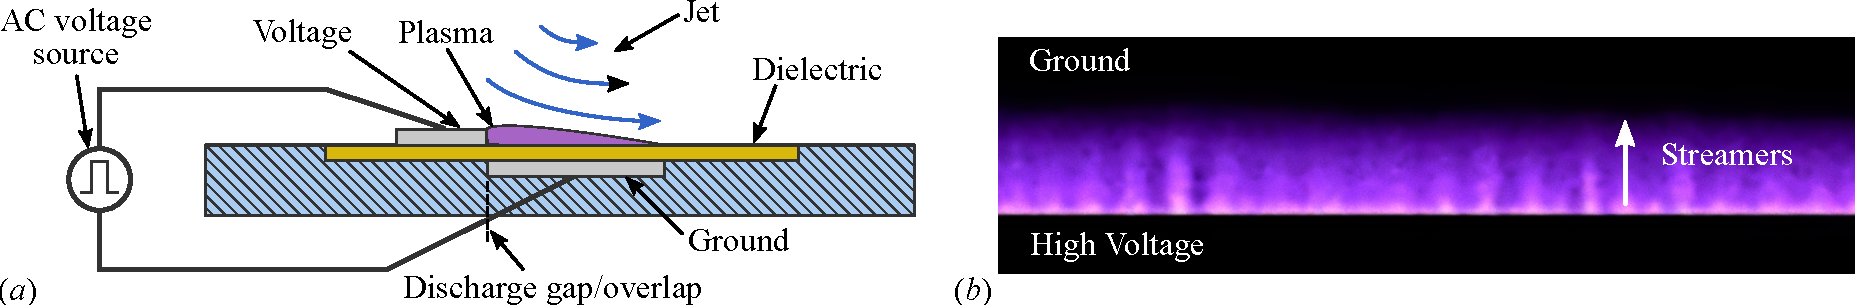
\includegraphics[width = 0.99\linewidth]{figures/schematic_plasma.pdf}
    \caption{AC-DBD plasma actuator. (a) Schematic of a typical cross-section of an asymmetric AC-DBD plasma actuator. (b) Top-view photograph of the purple glow on a DBD plasma actuator.}
    \label{fig:schematic_plasma}
\end{figure}

The specific dielectric-barrier-discharge configuration consists of two electrodes separated by a dielectric material. One of the electrodes is referred to as \textit{encapsulated}, which is commonly grounded and covered by the dielectric material. The remaining electrode is known as \textit{exposed}, since it is in direct contact with the surrounding fluid. The latter is connected to a high-voltage supply that is used to reach the breakdown voltage to generate plasma. Note, however that the opposite configuration with a high-voltage \textit{encapsulated} electrode and a grounded \textit{exposed} electrode is also possible. For a single plasma actuator configuration in which only one plasma plume is produced, the electrodes arrange as shown in figure~\ref{fig:schematic_plasma}(a). Upon the application of high voltage (HV), charge tends to accumulate on the surface of the dielectric material, yielding filamentary micro discharges, also known as streamers \citep{Kogelschatz2002filamentary} (figure~\ref{fig:schematic_plasma},b). These streamers change the capacitance of the dielectric barrier, reversing the local electric field and, thus, terminating themselves \citep{Eliasson1991streamers}. Based on this phenomenon, a continuous plasma discharge requires the application of variable voltage, either in the alternating or pulsating form \citep{michelis2017boundary}. Although the application of DC voltage is possible by substituting the dielectric barrier with a resistive barrier \citep{Laroussi2002resistive}, the most typical configuration of DBD actuators employs AC voltage, as shown in figure~\ref{fig:schematic_plasma}. For an AC-DBD plasma actuator working in air, the plasma is characterised by the back-and-forth motion of heavy ions, following the AC polarity inversion. This motion promotes collisions among the heavy-charged species (positive and negative ions), which results in a momentum exchange with the surrounding air \citep{Kotsonis2015review}. The resultant electric field and, thus, discharge are asymmetric due to the electrode arrangement. Consequently, the momentum exchange produces an uneven body force that directs from the exposed to the covered electrode, which induces a wall-tangent motion of the fluid. The resultant wall-jet structure, also referred to as \textit{ionic wind} \citep{Benard2014review}, injects fluid at a velocity which does not typically exceed $10\mathrm{m/s}$ \citep{Moreau2007review}.

Flow control strategies based on plasma actuators received much interest during the last few decades, still being very promising due to their electric nature. As the Aristotelian \textit{unmoved mover}, plasma actuators do not need movable parts to induce a fluid motion. At the same time, these devices feature a high-frequency response, being fully controllable in terms of amplitude and frequency within their operating limits. From a practical standpoint, plasma actuators require low power to operate, and their manufacturing is rather simple. In addition, they are very versatile in terms of geometrical patterns, extension, and thickness, which makes them very suitable to be flush-mounted devices with minimal flow disturbance while inducing body forces in the desired region direction and shape. Besides their control authority restricting their application to high Reynolds numbers, the aforementioned factors make DBD plasma actuators good choices for controlling aerodynamic flows such as laminar-to-turbulent transition \citep{Grundmann2008cancelTS,kotsonis2015control} and separation \citep{Little2010airfoilplasma,Michelis2015track}. A thorough summary of flow control studies based on DBD-plasma actuators is provided by the extensive reviews by \citet{Moreau2007review}, \citet{Corke2010}, \citet{Benard2014review}, and \citet{Kotsonis2015review}.

Plasma actuators have also been used to control the momentum fluxes within turbulent flows, especially for skin-friction reduction. A common approach consists of inducing spanwise travelling waves or spanwise oscillations. This strategy relies on the classic drag-reduction methodology proposed by \citet{Schoppa1998}, which aims at generating streamwise vortices embedded in a boundary layer to reduce momentum fluxes at the wall. In this regard, the experimental study of \citet{Whalley2014} employs a set of different plasma actuators to investigate the effect of co- and counter-rotating streamwise vortices in a turbulent boundary layer. They conclude that the formation of the spanwise travelling wave enables the formation of wide ribbons of low-speed streamwise velocity within the viscous sublayer, which locally reduces skin friction. Likewise, \citet{jukes2006TBLcontrol} achieved a strong skin-friction drag reduction downstream of the plasma actuator. These so-called ``plasma streamwise vortex generators'' (PSVGs) consist of a single or an array of plasma actuators aligned with the flow direction. Hence, the momentum injection by the actuators is normal to the mainstream, which leads to twisting and folding of the flow that eventually transforms into a streamwise vortex \citep{jukes2013plasmaVG}. The use of streamwise-aligned plasma actuators has been investigated in laminar \citep[e.g.,][]{jukes2013plasmaVG,serpieri2017} and turbulent boundary layers \citep[e.g.,][]{Jukes2006, Whalley2010DBDvortex, Wittig2019VGplasma} with promising results as a skin-friction drag reduction technique. 

Regarding heat transfer control, DBD plasma actuator applications are rather unexplored. It is worth noting that, despite the non-thermal nature of cold plasma, the plasma discharge locally produces thermal energy that may lead to a thermal footprint. Nonetheless, most of the produced heat diffuses through the dielectric and is not released to the fluid flow \citep{Rodrigues2018,Jukes2006}. The DBD plasma actuator proposed in this thesis resembles to that studied by \citet{Whalley2014}, \citet{Wittig2019VGplasma}, and, especially, \citet{cheng_wong_hussain_schroder_zhou_2021} (see figure~\ref{fig:dbd_actuator}). According to \citet{Wicks2015}, for opposing plasma discharges, streamwise vorticity generates upon the re-orientation of wall-normal vorticity from the actuators and spanwise vorticity from the boundary-layer, towards the streamwise direction. The reason behind this choice is that, contrary to conventional spanwise-aligned actuators, injecting momentum in the free stream direction to energise or weaken the boundary layer, the generation of streamwise vortices could potentially reduce turbulent fluxes at the wall. The research in Paper 2 thus aims at reducing convective heat transfer with an array of plasma actuators streamwise vortex generators. 

\begin{figure}
    \centering
    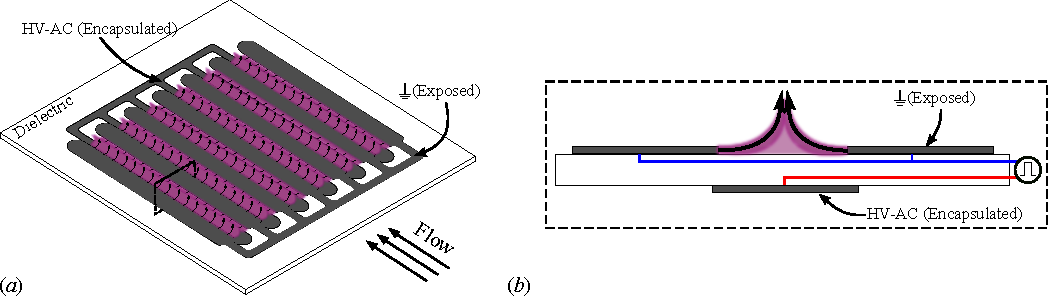
\includegraphics[width = 0.99\linewidth]{figures/dbd_actuator.pdf}
    \caption{Schematic representation of the DBD-plasma actuator array used in Paper 2. (a) Tri-dimensional representation of the array, and (b) cross-section of a pair of actuators.}
    \label{fig:dbd_actuator}
\end{figure}

As shown in figure~\ref{fig:dbd_actuator}, an array of DBD plasma actuators is considered in this thesis. Each actuator shares the encapsulated electrode with its adjacent. A total of 6 linear bi-directional actuators is used to ensure spanwise uniformity of the plasma-induced control. In this particular case, the air-exposed electrode is grounded while the encapsulated electrode beneath the dielectric material is connected to a stable high-voltage supply. As described in Paper 2 of this thesis, the actuator generates a sequence of opposing wall jets tangent to the surface in the spanwise direction, inducing pairs of counter-rotating streamwise vortices. In the recent study by \citet{cheng_wong_hussain_schroder_zhou_2021}, pairs of streamwise counter-rotating vortices are induced by plasma, merging with natural TBL streaks and interrupting the turbulence regeneration cycle, thus reducing skin friction. Invoking Reynolds' analogy of momentum and energy fluxes in turbulent boundary layers, the methodology proposed in Paper 2 exploits the same principles for an effective reduction of convective heat transfer in a turbulent boundary layer.

%------------------------------------------------------------------------------------------
\subsection{Jets in crossflow}\label{ss:JICF}

The jet in crossflow (JICF), or transverse jet, is a complex flow configuration present far and wide in natural processes and engineering applications. It is possible to find JICF in natural phenomena such as volcanic eruptions or the merge of a river and its tributary, although they are most commonly studied due to their relevance in the engineering field like for film cooling of turbine blades or thrust vector control for missiles, to name a few. Thus, the jet in crossflow can be adapted to the application, with several possible alternatives in nozzle size and shape, pulsation, inclination of the injection plane or injected fluid, for instance. The extensive field of application and variations of JICF requires a deep understanding of the flow topology, mixing, structural and sometimes reactive features to accurately design the operating and control conditions \citep{Karagozian2014revJICF}.

The utilisation of transverse jets for flow control is still an active research field with constant technological development and practical applications. It is well-agreed that a jet stream interacting with a crossflow provides better mixing capabilities than a free jet or a mixing layer \citep{kamotani1972experiments, broadwell1984structure}. The complex interaction of the jet flow with the freestream induces a web of flow structures and vortex systems that must be properly understood and managed for an effective flow-control purpose. The canonical configuration of a steady round jet perpendicular to a crossflow has been widely studied in the last decades \citep{kamotani1972experiments, fric_roshko_1994, kelso1996experimental, broadwell1984structure, smith1998mixing} due to its relevance in several engineering fields, especially in air-breathing engines. 

Following the seminal research work by \citet{fric_roshko_1994} and the extensive reviews by \citet{Mahesh2013revJICF} and \citet{Karagozian2014revJICF}, four main vortical structures are distinguished, as illustrated in figure~\ref{fig:JICF}. Upon the interaction of the freestream flow with the jet stream, small coherent structures develop in the form of ring-like vortices, commonly known as shear-layer vortices, which dominate the upstream formation of the jet column and are found to have the same direction of vorticity and similar length scales as the boundary layer formed inside the jet. These vortical structures are said to be formed from instabilities in the jet's shear layer, particularly on Kelvin-Helmholtz instabilities near the jet exit \citep{fric_roshko_1994, kelso1996experimental}. It is worth noting that the jet shear-layer instability found on free and transverse jets are significantly different in nature and formation characteristics \citep{megerian2007transverse}. Second, dominating the jet cross-section, a counter-rotating vortex pair (CVP) is produced in the near-field region of the jet \citep{kamotani1972experiments}. This large vortical structure is responsible for the pressure difference between the downstream and upstream sides of the jet exit and the vorticity evolution in the shear layer of the jet stream \citep{andreopoulos1984experimental, cortelezzi2001formation}. The formation of the CVP is attributed to the roll-up of vortex rings in the near-field region of the flow. The interaction among the vortex rings, as well as their roll-up and deformation, can be influenced by changes in flow conditions, such as the crossflow velocity, jet velocity and boundary layer thickness and have a significant impact on the entrainment of the crossflow into the near-field of the jet \citep{smith1998mixing,kamotani1972experiments,cortelezzi2001formation}. Third, a system of horseshoe vortices wraps around the jet base \citep{Krothapalli1990HSvort} due to the interaction between the mainstream boundary layer and the transverse flow exiting the jet \citep{kelso1995horseshoe}. These trailing vortices resemble those formed in flows around wall-mounted cylinders but can also oscillate and coalesce with other structures in the flow, leading to an unsteady regime under certain flow conditions \citep{kelso1995horseshoe}. Last, smaller-scale structures build up downstream of the jet column primarily attached to the wall and contain fluid of the wall boundary layer that entrains into the jet stream \citep{fric_roshko_1994}. The formation mechanism of the wake vortices is fundamentally different from those found in the flow around solid cylinders as the vortices are not shed directly from the jet but originate in the wall boundary layer. Periodic separation of the wall boundary layer caused by adverse pressure gradients induces an upward release of fluid and vorticity that generates column-like structures rising from the wall \citep{fric_roshko_1994}. These coherent structures contribute to the transverse jet's complex structure and mixing characteristics \citep{smith1998mixing}. The horseshoe vortex and the CVP, in particular, play a key role since they add to the mean flow while the wake and shear vortices mainly affect the fluctuating dynamics of the jet \citep{karagozian1986analytical}.

\begin{figure}
    \centering
    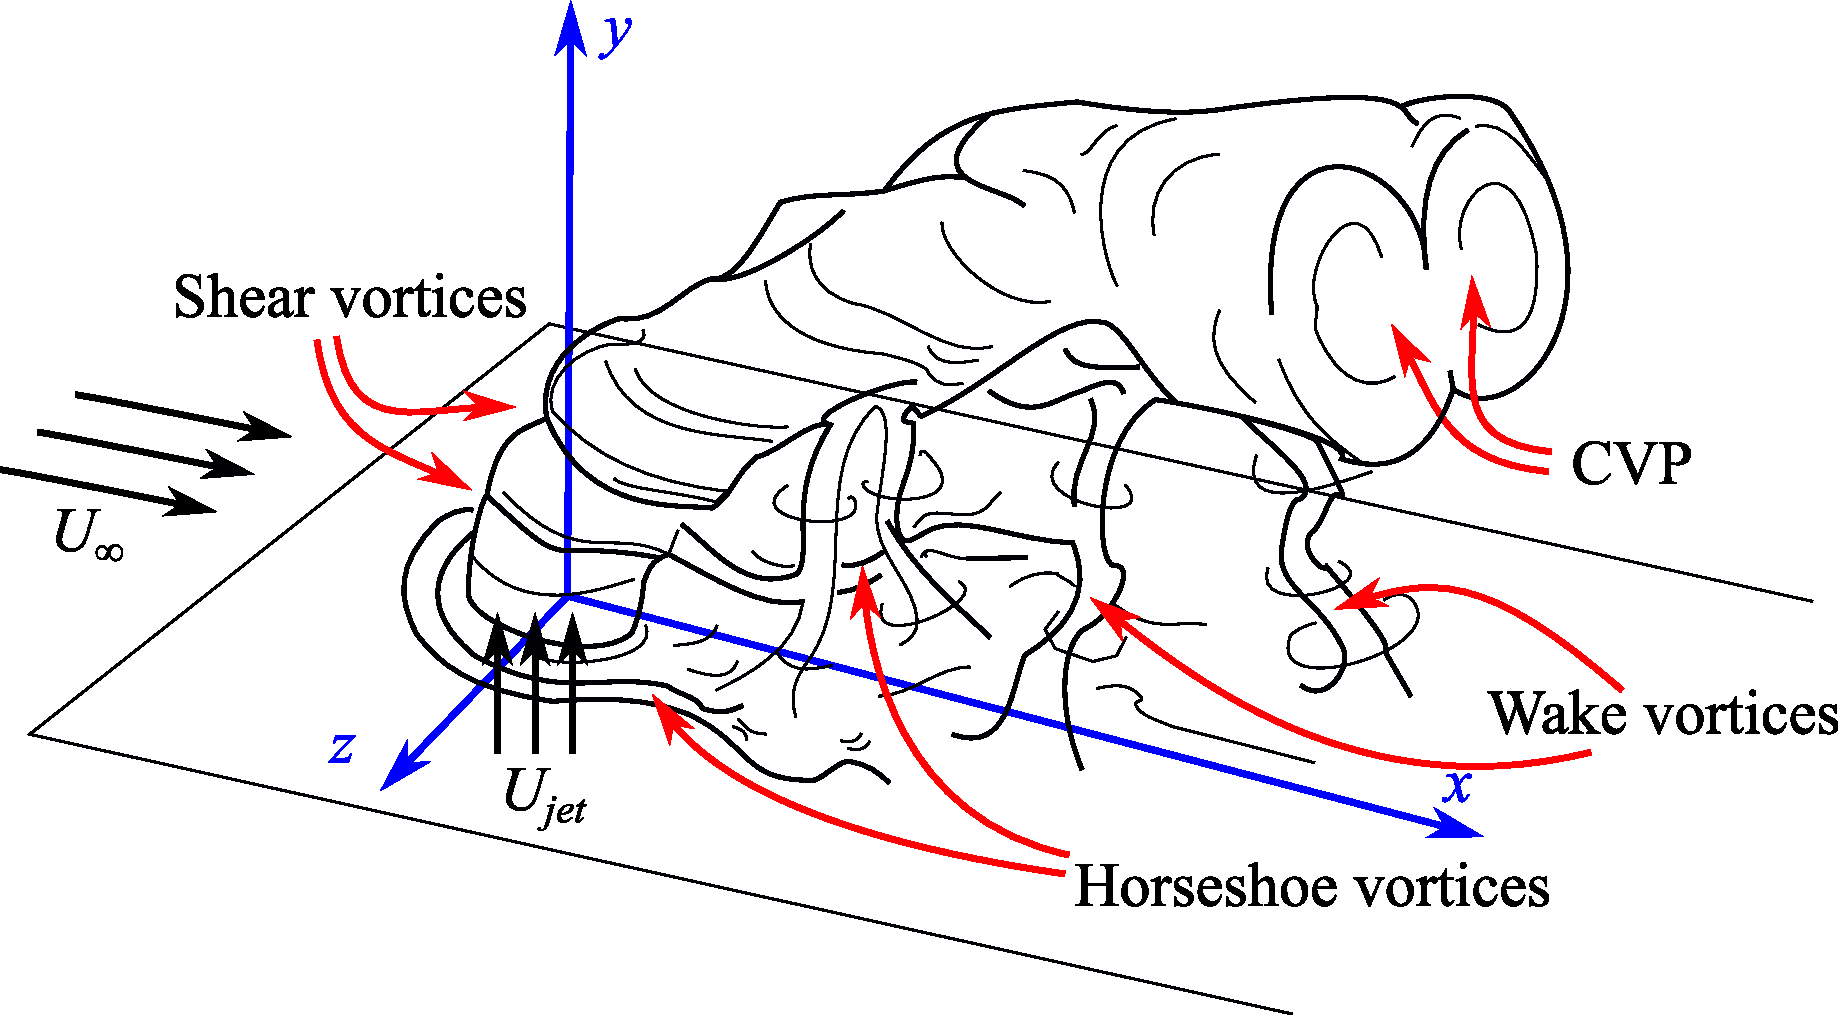
\includegraphics[width = 0.7\linewidth]{figures/JICF.pdf}
    \caption{Vortical structures for a round jet injecting steady fluid into a normal crossflow. Adapted from \citet{Karagozian2014revJICF}.}
    \label{fig:JICF}
\end{figure}

The mixing enhancement is the most common target when the JICF is used as a flow control actuator. This application is reported in the classic work by \citet{smith1998mixing}, which shows that the mixing enhancement narrows to the near-field region of the flow dominated by the CVP's structural formation and not to the far-field region where the CVP is fully developed. Regarding heat transfer enhancement applications, \citet{puzu2019jet} investigated the influence of the CVP and horseshoe vortices downstream of the jet injection. They report that the secondary mixing by the combined effect of the collapse of the CVP and the merge of the horseshoe vortices leads to a local convective heat transfer enhancement due to better entrainment and mixing within the boundary layer. Nonetheless, there is consensus that the pulsation or modulation of the JICF considerably improves its mixing performance compared to the steady jet. This matter is discussed in the experiments by \citet{vermeulen1992mixing, johari1999penetration, eroglu2001structure, MCLOSKEY2002, Johari2006scaling}, to name a few. \citet{vermeulen1992mixing} reported a considerable increase in the mixing area, penetration, and overall mixing by acoustically exciting a jet into a hot crossflow. They also concluded that the collapse of the structures and the interaction promoting mixing are displaced upstream, with higher mixing rates in the downstream vicinity of the injection. On the other hand, \citet{johari1999penetration} considered a fully-modulated JICF (valve-actuated) to study the effect of the frequency and duty cycle on the mixing properties, demonstrating that a short injection time (also referred to as pulse width) provides a higher mixing performance and dilution. The experiments by \citet{eroglu2001structure} and \citet{MCLOSKEY2002} focus on the induced perturbations on the vortical structures by the pulsation, finding that square-wave excitation generates distinct vortex rings. Most of the investigations of flow control with pulsed JICF agree on the importance of tuning the control strategy to find the optimal configuration that amplifies or optimises the desired flow feature \citep{shapiro2006optimization}. However, there is no universal objective function to drive the optimisation of pulsation due to the dependency on the flow and pulsation conditions, which are found to be apparatus-dependant \citep{MCLOSKEY2002}. The interested reader is referred to the extensive review article by \citet{karagozian2010transverse} covering the jet in crossflow and its control.

Besides the undeniable suitability of pulsed JICF for several flow control applications, there is still a profound lack of consensus on the flow structures, the dynamics and the correct scaling that characterise this flow configuration \citep{Sau2010optJICF}. The \textit{formation number} \citep{gharib1998scalingVR} is used in some studies \citep[e.g.][]{MCLOSKEY2002,shapiro2006optimization} to express the optimal pulsation condition, although this parameter was conceived for quiescent flows. \citet{Johari2006scaling} proposes the \textit{stroke ratio} and \textit{duty cycle} to scale the pulsed JICF together with a classification of induced structures such as hairpin vortices, vortex rings with or without trailing columns or turbulent puffs; nonetheless, \citet{Sau2008dynamicsVRICF} refuted this idea, demonstrating its validity just for quiescent flow conditions. The regime map suggested by \citet{Sau2010optJICF} builds upon two dimensionless parameters, namely the \textit{ring velocity ratio} and the \textit{stroke ratio}, gathering the effects of the pulsation frequency, duty cycle, modulation, and pulsed energy. For small ring velocity ratios, i.e. low injection velocities compared to the crossflow, the induced structures develop as hairpin vortices that progressively get closer as the stroke ratio is increased. There are two possibilities for high values of the ring velocity ratio: isolated vortex rings and vortex rings followed by a trailing column of vorticity, which depend on a low or high value of the stroke ratio, respectively. This map seems to reasonably fit with previous existing literature, showing that the optimal pulsation of JICF may be explained in terms of their vortex rings and that the optimal experimental conditions are seen to collapse on the same optimal curve. Howbeit, most of the engineering and technological studies that explore the utilization of pulsed JICF get behind the Strouhal number, $\mathrm{St}$, to characterise the modulation of the jet. In this regard, Paper 3 and Paper 5 of this thesis rely on the duty cycle and the Strouhal number as the scaling parameters to define the control action.

A simplified schematic of the pneumatic system used in Paper 3 and Paper 5 to generate the JICF is illustrated in figure~\ref{fig:schematic_pneumatic}. A pressurised air supply provides the jet stream. The air is filtered to avoid spurious oil or solid particles from entering the experimental setup. The control of the jet stream is performed in two steps. First, a pressure relief valve controls the absolute pressure on the system, which is always lower than that provided by the air compressor. This condition guarantees a constant operating pressure regardless of the jet actuation parameters. Second, a flowmeter and controller are used to monitor the flow condition, namely mass and volumetric flow rates, temperature, density and pressure. A settling chamber is used to prevent the flow meter and the pressure relief valve from spurious pressure waves induced by the ram effect at the solenoid valve. Eventually, a slot jet diffuser is used to progressively transition from a round shape of the pressurized line to the final rectangular shape at the jet exit.

\begin{figure}
    \centering
    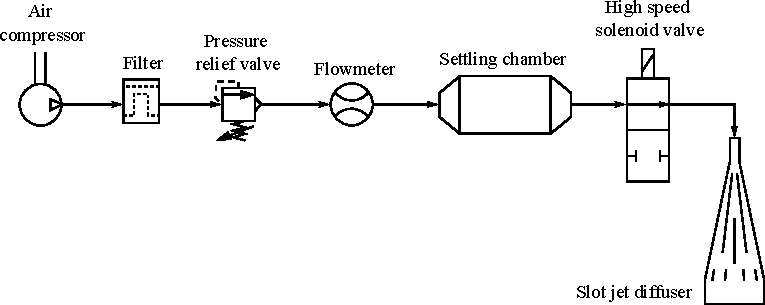
\includegraphics[width = 0.95\linewidth]{figures/schematic_pneumatic.pdf}
    \caption{Schematic of the experimental apparatus to control the jet in crossflow in the investigations of Paper 3 and Paper 5.}
    \label{fig:schematic_pneumatic}
\end{figure}

The dynamical behaviour and the flow topology of a non-circular JICF are very similar to those described above \citep{liscinsky1996crossflow, plesniak2005scalar}, especially in the far-field region of the flow. The interested reader is referred to the classic review by \citet{Gutmark1999noncirc}, where several investigations of flow control with non-circular jets are reported. In particular, the spanwise slot JICF has been investigated both experimentally and numerically for the steady-blowing configuration, and with jet modulation \citep[see e.g.][]{park1999, Krogstad2000slitjet, steinfurth2021CFslot}. The recent series of studies of pulsed slot jets in quiescent flow conditions \citep{steinfurth2020quiescentslot}, normal to a crossflow \citep{steinfurth2021CFslot}, and with an inclination angle of the injection plane with respect to the crossflow \citep{Steinfurth2021pulsedjet} shed some light on the flow structures for this kind of geometry. The flow configuration in Paper 3 resembles that investigated by \citet{Steinfurth2021pulsedjet}, in which the spanwise slot jet injects air at $30^\circ$ with respect to the wall. The inclination yields the jet stream to remain attached to the wall due to a Coand\v{a} effect and a local pressure deficit. A leading vortex develops downstream of the wall-attached jet, which eventually transforms into a half-ring vortex. On the other hand, the configuration used in Paper 5 looks like that in \citet{cheng2021skin} which combines several slot jets aligned with the freestream to promote skin-friction reduction in a turbulent boundary layer. 

\clearpage \newpage
\ \thispagestyle{empty}